\section{実験装置}

\subsection{熱プレス機}
板材の成形は小型熱プレス機(アズワン AH-1TC)を用いて行った.熱線の入った金属板で荷重を加えながら対象物を挟むことによって,所望の温度・荷重にて対象物を保持することができる.通常,対象物はペレット等の元となる材料を型に敷き詰めたものであり,温度が上昇することによってペレットが溶け,荷重が加えられて型に流れ込むことで試料が作製される.

\subsection{引張試験機}
材料の力学特性を測定するのに一般的に行われるのが引張試験である.この試験では棒状の試料に引張荷重を付与することによって荷重と棒の伸びの関係を計測し,それらを応力とひずみの関係に変換した.引張試験には万能試験機(東洋精機製ストログラフVG20 kN)を用いた.

\subsection{偏光顕微鏡}
図\ref{fig:光学系}に偏光顕微鏡の光学系を示す.試料の下に光源がある場合,試料の上下にそれぞれ偏光子および検光子と呼ばれる偏光板が配置される.偏光子および検光子を透過した直線偏光の振動面が直行する状態を直交ニコルと呼び,この状態において偏光顕微鏡のステージに試料が無い場合は暗視野となる。一方,直交ニコルの状態で結晶性高分子を偏光顕微鏡(KEYENCE デジタルマイクロスコープVHX-6000)のステージに置くと,図\ref{fig:球晶構造}のような結晶組織が観察できる.

\begin{figure}[htbp]
    \centering %中央揃え
    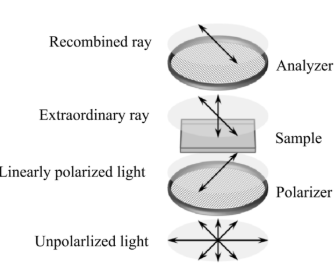
\includegraphics[width=100truemm,clip]{fig/fig_光学系.png}
    \caption{Optics of Polarizing Microscope.}
    \label{fig:光学系}
\end{figure}